% Lecture file created by newnote
% Class: Models of Theoretical Physics
% Professor: Azaele Sandro
% Date: 2025-10-17
\lecture{1}{ODEs from reaction rates}{2025-10-17}
\pagelayout{margin}
% --- Start writing here ---

\section{ODEs from reaction rates}
Chemical reactions form a broad field of applications where deterministic and stochastic methods are very useful. Such reactions include a wide class of systems where individuals of some entity encounter randomly and then react with some others of the same or different entity (reactants) and produce individuals which may be of a different nature (products) w.r.t. the reactants. The systems that can be studied in this framework include:

\begin{enumerate}
    \item Actual chemical reactions which involve particles on molecules which transform upon collisions.
    \item Population systems, where individuals may die, give birth, mate, consume each other, immigrate....
    \item Epidemics, where diseases are transmitted from ind. to ind. (infected \& susceptibles)
    \item Gene expression, where genes can be transcribed (into mRNA) and translated (into proteins) upon the appropriate occurrence of some transcription factors.
    \item ...
\end{enumerate}

These reactions may be reversible or not, according to whether the direct reaction can also occur in the backward direction.

In this part of the module we will be only concerned with the deterministic properties of these systems (mean-field approx.), namely, we will not study their stochastic properties.

We will write down the ODEs for the concentrations of the reactants and products starting from the corresponding rules that govern the chemical reactions.

\subsection*{Binary and irreversible reaction}
A molecule of type $X$ and a molecule of type $Y$ (reactants) collide and react to produce a molecule of type $Z$ (product):
\begin{DispWithArrows}
    x+y \xrightarrow{k} z \tag{1}
\end{DispWithArrows}
$K$ is the kinetic constant which is used to compute $r(x, y)$, which gives the rate of occurrence of the reaction
\begin{DispWithArrows}
    2 \mathrm{H}_{2}+\mathrm{O}_{2} \xrightarrow{\mathrm{~K}} 2 \mathrm{H}_{2} \mathrm{O}
\end{DispWithArrows}
stoichiometric coefficients: # of react. or prod. of each type that are consumed or produced in the reaction.

\subsection*{Calculation of the reaction rate}
We assume that the reaction occurs in a finite volume $V$ where the molecules are well-stirred and the concentrations of $X, Y$ and $Z$ are "small", despite the number of molecules of each type is "large". We will assume that the concentrations $x=\frac{n_{x}}{v}, y=\frac{n_{y}}{v}, z=\frac{n_{z}}{v}$ ( $n_{i}$ : # of molec. of type $i$ ) are continuous variables. We want to estimate $r(x, y)$, the reaction rate, in the diluted limit case:
\begin{DispWithArrows}
    r(x, y) \simeq r(0,0)+\left(\partial_{x} r_{0}\right) x+\left(\partial_{y} r_{0}\right) y+\left(\frac{1}{2} \partial_{x x}^{2} r_{0}\right) x^{2}+\left(\partial_{x y}^{2} r_{0}\right) x y+\left(\frac{1}{2} \partial_{y y}^{2} r_{0}\right) y^{2}+h_{0} t \tag{2}
\end{DispWithArrows}
small concentrations $x, y$
We expect that $r(0, y)=0$ for all $y$ as well as $r(x, 0)=0$ for all $x$, because we need both $x$ and $y$ for the reaction to occur. Therefore from eq. (2) we get
$r(0, y)=r(0,0)+\left(\partial_{y} r_{0}\right) y+\left(\frac{1}{2} \partial_{y y}^{2} r_{0}\right) y^{2} \equiv 0 \quad \Rightarrow r(0,0)=0, \partial_{y} r_{0}=0, \partial_{y y}^{2} r_{0}=0$
$r(0, x)=\partial_{x} r_{0} x+\frac{1}{2} \partial_{x x}^{2} r_{0} x^{2} \equiv 0 \Rightarrow \partial_{x} r_{0}=0, \partial_{x x}^{2} r_{0}=0$
Hence we are left with
\begin{DispWithArrows}
    r(x, y)=\partial_{x y}^{2} r_{0} x y \equiv k x y \tag{3}
\end{DispWithArrows}
Obs: particles are free to move and randomly meet with each other: the prob. of $x$ and $y$ to collide are indip. When they meet, they can react.
where the kinetic constant $k$ does not depend on concentrations. $k$ may depend on the temperature, $k=k_{0} e^{-\frac{E}{k T}}$ (E activation energy), with the Arrhenius factor $e^{-E / k T}$.

The previous motivation leads to an approximate/empirical "law" which is simple and useful in many situations:

\subsection*{The law of Mass Action}
In a first approximation, the rate of any chemical reaction is proportional to the product of the concentrations of the reacting substances.

We can use this law to deduce the ODEs for the evolution of the concentrations. If we know the concent. at time $t$, then at time $t+\Delta t$ (see eq.(1)):
\begin{DispWithArrows}
    \begin{aligned}
    & x(t+\Delta t)=x(t)-k x(t) y(t) \Delta t \\
    & y(t+\Delta t)=y(t)-k x(t) y(t) \Delta t \\
    & z(t+\Delta t)=z(t)+k x(t) y(t) \Delta t
    \end{aligned} \quad \xrightarrow{\Delta t \to 0}\left\{\begin{array}{l}
    \dot{x}=-k x y, x(0)=x_{0} \\
    \dot{y}=-k x y, y(0)=y_{0} \\
    \dot{z}=k x y, z(0)=z_{0}
    \end{array}\right. \tag{4}
\end{DispWithArrows}
Eq. (4) has a conservation law:
$\dot{x}-\dot{y}=0 \quad \Rightarrow \quad x(t)-y(t)=x_{0}-y_{0}=c$ constant Therefore we can simplify eq. (4):

\begin{figure}[H]
    \centering
    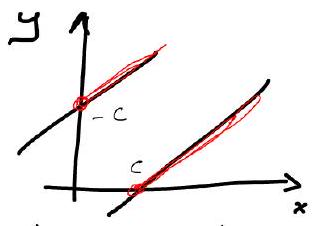
\includegraphics[width=\textwidth]{2025_10_17_109d3ce1ba98c27731a1g-3}
\end{figure}

\begin{DispWithArrows}
    \dot{x}=-k x(x-c)=k x(c-x) \tag{5}
\end{DispWithArrows}
This is called logistic equation and can be solved analytically:
\begin{DispWithArrows}
    x(t)=\frac{c x_{0} e^{c k t}}{c+x_{0}\left(e^{c k t}-1\right)} \tag{6}
\end{DispWithArrows}
\begin{figure}[H]
    \centering
    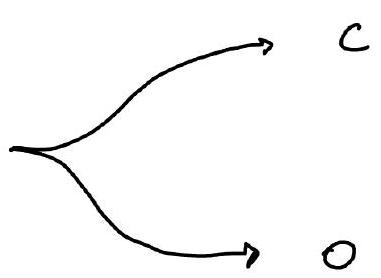
\includegraphics[width=0.5\textwidth]{2025_10_17_109d3ce1ba98c27731a1g-3(1)}
    \caption{if $c>0$ as $t \rightarrow+\infty$}
\end{figure}
if $c<0$

Check of (6) out. What happens if $c=0$? Solve eq. (4) for $z(t)$. There is another independent conservation law: $\dot{x}+\dot{z}=0 \Rightarrow x(t)+z(t)=x_{0}+z_{0}$ Therefore if $c>0, z \longrightarrow x_{0}+z_{0}-c=z_{0}+y_{0}$ as $t \rightarrow \infty$; all $y$ goes to $z$. If $c<0, z \rightarrow z_{0}+x_{0}$.

\begin{figure}[H]
    \centering
    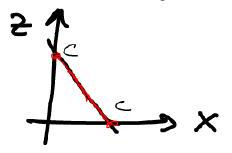
\includegraphics[width=\textwidth]{2025_10_17_109d3ce1ba98c27731a1g-3(2)}
\end{figure}

\subsection*{Binary reversible reaction:}
\begin{DispWithArrows}
    x+y \underset{k_{-}}{\stackrel{k_{+}}{\rightleftarrows}} z \quad k_{ \pm}>0 \tag{7}
\end{DispWithArrows}
Along the same lines as before we deduce the evolution of concent.
\begin{DispWithArrows}
    \left\{ \begin{array} {l}
    \dot{x}=k_{-}z-k_{+}x y \\
    \dot{y}=k_{-}z-k_{+}x y \\
    \dot{z}=-k_{-}z+k_{+}x y
    \end{array}\right. \tag{8}
\end{DispWithArrows}
Verify that there are two independent conservation laws $x(t)-y(t)=c_{1}$, and $x(t)+z(t)=c_{2}$. Hence the eq. for $x$ can be written as
\begin{DispWithArrows}
    \dot{x}=k_{+} x\left(c_{1}-x\right)+k_{-}\left(c_{2}-xight) \tag{9}
\end{DispWithArrows}
Obs: even this eq. can be solved analytically.

A more complicated case: the Haber process. This process was developed by F. Haber in the early '900s for producing ammonia on an industrial scale: $N_{2}($ nitrogen $)+3 H_{2}($ hydrogen $) \longrightarrow 2 NH_{3}$ (ammonia) We consider then the reaction:
\begin{DispWithArrows}
    X+3 Y \underset{k_{-}}{\stackrel{k_{+}}{\rightleftarrows}} 2 z \tag{10}
\end{DispWithArrows}
The ODEs for the concentrations are then:
\begin{DispWithArrows}
    \left\{\begin{array}{l}
    \dot{x}=-k_{+} x y^{3}+k_{-} z^{2} \\
    \dot{y}=-3 k_{+} x y^{3}+3 k_{-} z^{2} \\
    \dot{z}=-2 k_{-} z^{2}+2 k_{+} x y^{3}
    \end{array}\right. \tag{11}
\end{DispWithArrows}
The stoichiometric coefficients enter the ODEs:
Let's interpret the term $-3 k_{+} x y^{3}$ in eq. (11b)

Eq. (10) tells us that 3 molecules (or moles) of $Y$ have to collide independently along with one molecule (or mole) of $X$ for the reaction to occur in the forward (+) direction. Also, because for every molecule of $X$, three molecules of $Y$ react, for a decrease in concentration of $x$, there is a three fold decrease in concentration of $Y$. Thus, the stoichiometric coefficients affect the prob. of a reaction to occur as well as the relative speed of the reaction. Indeed, $3 \dot{x}=\dot{y}$, which relates the two speeds of reaction.
The term $3 k_{-}z^{2}$ has a similar interpretation: for producing $Y$, two molecules (moles) of $Z$ have to collide which will generate 3 molec. of $Y$. Also, for every 2 molec. of $z$ that decompose in the backward direction ($k_{-}$), there will be 3 molec. of $Y$. This means that the speeds of reaction are $3|\dot{z}|=2|\dot{y}|$. If we look at eq. 11.b,c we get $3 \dot{z}=-2 \dot{y}$ because the decrease of $Y$ leads to an increase of $z$ and vice versa.

Obs: at stationarity $\frac{x y^{3}}{z^{2}}=\frac{k_{-}}{k_{+}}$, but there are also some conservation laws:
\begin{DispWithArrows}
    3 x(t)-y(t)=c_{1}, \quad 2 x(t)+z(t)=c_{2}, \quad 2 y(t)+3 z(t)=c_{3}
\end{DispWithArrows}
Can you see why these quantities are conserved and why $c_{1}, c_{2}$ and $c_{3}$ are not independent?

More generally, we can restate the law of mass action as

\subsection*{The law of Mass Action}
In a first approximation, the rate of any chemical reaction is proportional to the product of the concentration of the reacting substances, where every concentration is raised to a power equal to the corresponding stoichiometric coefficient which also has to be included in the reaction speed with the appropriate sign.

Ex: write down the rate equation for the reversible reaction in eq.(1)
\begin{DispWithArrows}
    2 \mathrm{H}_{2}+\mathrm{O}_{2} \underset{k_{-}}{\stackrel{k_{t}}{\rightleftarrows}} 2 \mathrm{H}_{2} \mathrm{O}
\end{DispWithArrows}
The general reaction
\begin{DispWithArrows}
    a X+b Y \underset{k_{-}}{\stackrel{k_{+}}{\rightleftarrows}} c z+d W \quad a, b, c, d \in \mathbb{N} \tag{12}
\end{DispWithArrows}
leads to the following odes:
\begin{DispWithArrows}
    \left\{\begin{array} {l}
    \dot{x}=a\left(-k_{+} x^{a} y^{b}+k_{-} z^{c} w^{d}\right) \\
    \dot{y}=b\left(-k_{+} x^{a} y^{b}+k_{-} z^{c} w^{d}\right) \\
    \dot{z}=c\left(+k_{+} x^{a} y^{b}-k_{-} z^{c} w^{d}\right) \\
    \dot{w}=d\left(+k_{+} x^{a} y^{b}-k_{-} z^{c} w^{d}\right)
    \end{array}\right.
\end{DispWithArrows}
Calculate the quantities that are conserved.
There are types of molecules or species that can interact in different kinds of reactions:
The predator $(Y)$ and prey $(X)$ system: (irreversible reactions)
\begin{DispWithArrows}
    \begin{aligned}
     X & \xrightarrow{k_{1}} 2 X \\
     Y+X & \xrightarrow{k_{2}} 2 Y \\
     Y & \xrightarrow{k_{3}} \phi
    \end{aligned} \tag{13}
\end{DispWithArrows}
reproduction of preys, predator eats a prey, predator dies.

To get the ODEs we have simply to sum the effects of different reactions:
\begin{DispWithArrows}
    \left\{\begin{array}{l}
    \dot{x}=k_{1} x-k_{2} x y \\
    \dot{y}=k_{2} x y-k_{3} y
    \end{array}\right. \tag{14}
\end{DispWithArrows}
These are the Lotka-Volterra equations. Show that at stationarity $\bar{x}=\frac{k_{3}}{k_{2}}, \bar{y}=\frac{k_{1}}{k_{2}}$ but the Jacobian at $(\bar{x}, \bar{y})$ has eigenvalues $\lambda= \pm i \sqrt{k_{1} k_{3}}$. Is the system stable? Show that $V(x, y)=k_{2}(x+y)-k_{3} \ln x-k_{1} \ln y$ is a conserved quantity.

\subsection*{General chemical reactions}
More generally we may consider $m$ different chemical species $x_{i}, i=1, 2 \ldots m$ which are involved in $n$ different reactions of the form
\begin{DispWithArrows}
    \sum_{i=1}^{m} a_{i j} X_{i} \underset{k_{j}^{-}}{\stackrel{k_{j}^{+}}{\rightleftarrows}} \sum_{i=1}^{m} b_{i j} X_{i} \quad j=1, 2, \ldots, n \tag{15}
\end{DispWithArrows}
where $a_{i j}$ and $b_{i j}$ are stoichiometric coefficients that are all non-negative integers.

Therefore the ODEs are
\begin{DispWithArrows}
    \dot{x}_{i}=\sum_{j=1}^{n}\left(b_{i j}-a_{i j}\right) r_{j}(\vec{x}) \quad i=1, 2, \ldots m \tag{16}
\end{DispWithArrows}
where $r_{j}(\bar{x}) \equiv k_{j}^{+} \prod_{i=1}^{m} x_{i}^{a_{i j}}-k_{j}^{-} \prod_{i=1}^{m} x_{i}^{b_{i j}} \quad$ for any $j=1, 2, \ldots, n$.
We want to find the conservation laws of eq. (16).
Let $S$ be the stoichiometric matrix: $S_{i j} \equiv b_{i j}-a_{i j}$ This is a $m \times n$ matrix.
In vector form eq. (16) reads
\begin{DispWithArrows}
    \frac{d}{d t} \vec{x}=S \vec{r}(\vec{x}) \tag{17}
\end{DispWithArrows}
A linear conserv. law for the system (15) or (16) has the form (if it exists)
\begin{DispWithArrows}
    \frac{d}{d t} \sum_{i=1}^{m} c_{i} x_{i}=0 \tag{18}
\end{DispWithArrows}
where $c_{i}$ are (not all zero) constants. If $\sum_{i} c_{i} x_{i}(t)$ is a constant of motion
\begin{DispWithArrows}
    \sum_{i} c_{i} x_{i}(t)=\sum_{i} c_{i} x_{i}(0)=\vec{c}^{\top} \cdot \vec{x}(0)
\end{DispWithArrows}
where $\vec{c}^{\top}=\left(c_{1}, c_{2}, \ldots, c_{m}\right)$. If we multiply eq (17) by $\vec{c}^{\top}$, then
\begin{DispWithArrows}
    \vec{c}^{\top} \cdot \frac{d}{d t} \vec{x}=\vec{c}^{\top} S \vec{r}(\vec{x})=0 \tag{19}
\end{DispWithArrows}
Eq. (19) holds true for all $\vec{r}$, hence it must be
\begin{DispWithArrows}
    \vec{c}^{\top} S=0 \quad \text { or } \quad S^{\top} \vec{c}=0 \tag{20}
\end{DispWithArrows}
The conservation laws of the system of reactions in eq - (16) are given by the non-zero elements $\vec{c} \in \operatorname{ker}\left(S^{\top}\right)$ ($\vec{c}^{\top} \cdot \vec{x}=\text{const}$) and the number of (linearly independent) conservation laws is given by $\operatorname{dim}\left(\operatorname{ker}\left(s^{\top}\right)\right)$. For the reaction $x+y \rightarrow z, S=\begin{pmatrix}-1 \ -1 \ 1\end{pmatrix}, \operatorname{ker}\left(S^{\top}\right)=\left\{\left(c_{1}, c_{2}, c_{3}\right) \mid c_{1}+c_{2}=c_{3}\right\}, \operatorname{dim}\[\operatorname{ker}\left(s^{\top}\right)\]=2$. $\sum_{i} c_{i} x_{i}=c_{1} x+c_{2} y+\left(c_{1}+c_{2}\right) z=\text { const. }$. Basis $(1,-1,0)$ and $(1,0,1) \rightarrow x-y=\text{const.}$
\begin{DispWithArrows}
    x+z=\text { const. }
\end{DispWithArrows}
Tools for the simulation of chemical reactions
Many tools and libraries are available for the numerical simulation of chemical reactions:

\begin{verbatim}
 http://copasi.org/                             COPASI                (free and professional)
 http://libroadrunner.org/                      LIBROADRUNNER         (for c++/Python)
 sbml.org/SBML_Software_Guide/SBML_Software_Summary                  (for a list)
\end{verbatim}

It is good practice to write down your own code for you to check whether you have understood the basics of the theory.

Also, these reactions should be implemented with stochastic algorithms which account for the discrete nature of the particles. These tools will be provided in the other part of the module.
